%preamble
\documentclass[letterpaper]{article}
\synctex=1
\usepackage{graphicx}
\graphicspath{ {images/} }

\usepackage{lipsum}
\usepackage{float}
% \bibliographystyle{IEEEtran}
% \bibliographystyle{ieeetr}

\usepackage{amssymb}

\usepackage{siunitx}

\usepackage{multirow}
% for merging table cells I think

\usepackage{fancyhdr} %header
\fancyhf{}
\fancyhead[R]{Arun Woosaree XXXXXXX}
\renewcommand\headrulewidth{0pt}
\fancyfoot[C]{\thepage}
\renewcommand\footrulewidth{0pt}
\pagestyle{fancy}

% make subsection use letters
\renewcommand{\thesubsection}{\thesection.\alph{subsection}}

%actual document
\begin{document}

% \maketitle %insert titlepage here
\begin{titlepage}
 \begin{center}
  \vspace*{1cm}
  \Huge
  Stat 235
  \vspace{1cm}
  
  Lab 1
  \vspace{1cm}
  
  By: Arun Woosaree
  \vspace{1cm}
  
  \Huge
  Lab EL12
  \vspace{1cm}
  
  TA: Jessa Marley
  \vspace{1cm}
  
  \today
  \vfill
 \end{center}
\end{titlepage}

\section{Histograms}

\subsection{Histograms of Thickness: 400ºC, 600ºC, and 800ºC}

\begin{figure}[H]
 \centering
 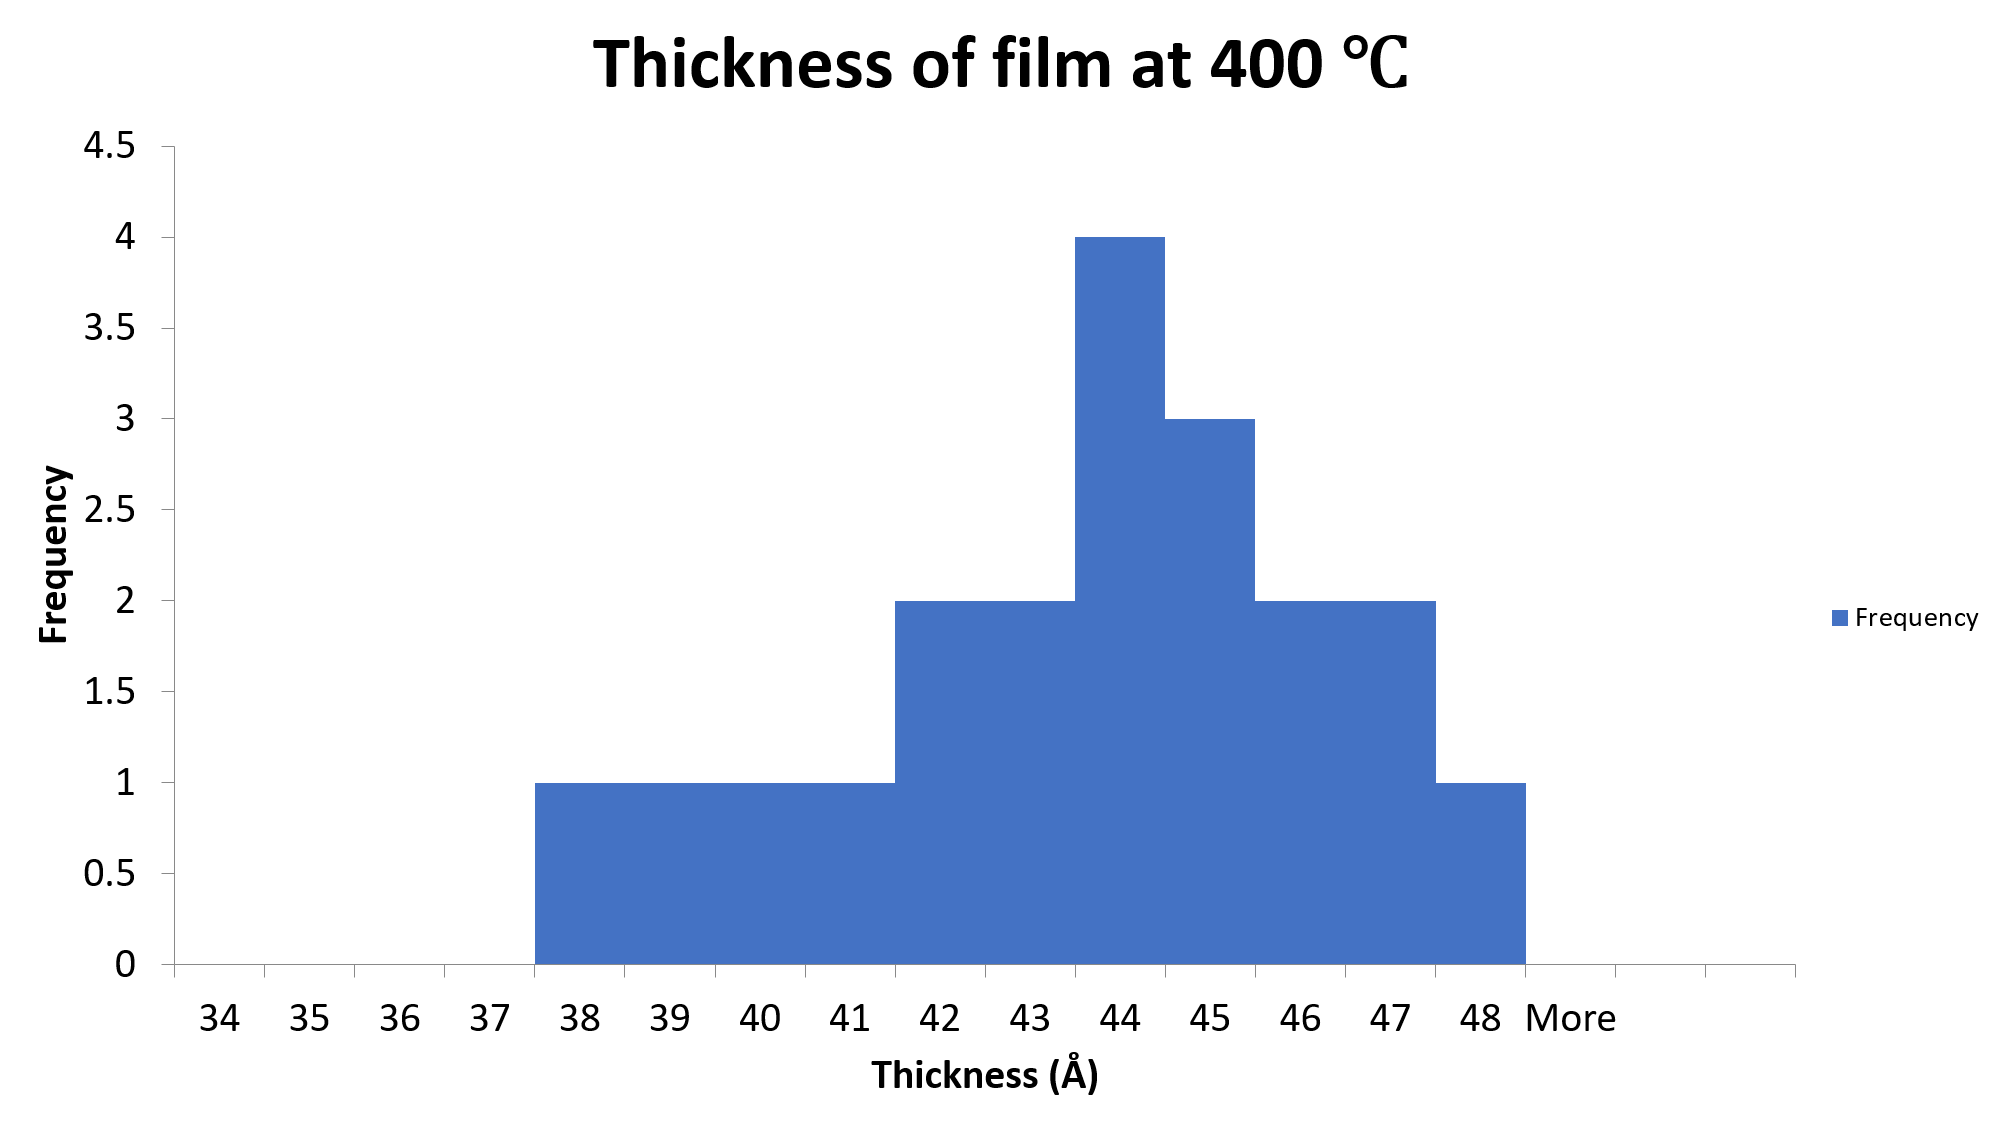
\includegraphics[width=\textwidth]{thicc400.png}
 \caption{INSERT CAPTION HERE}
 \label{thicc400}
\end{figure}

\begin{figure}[H]
 \centering
 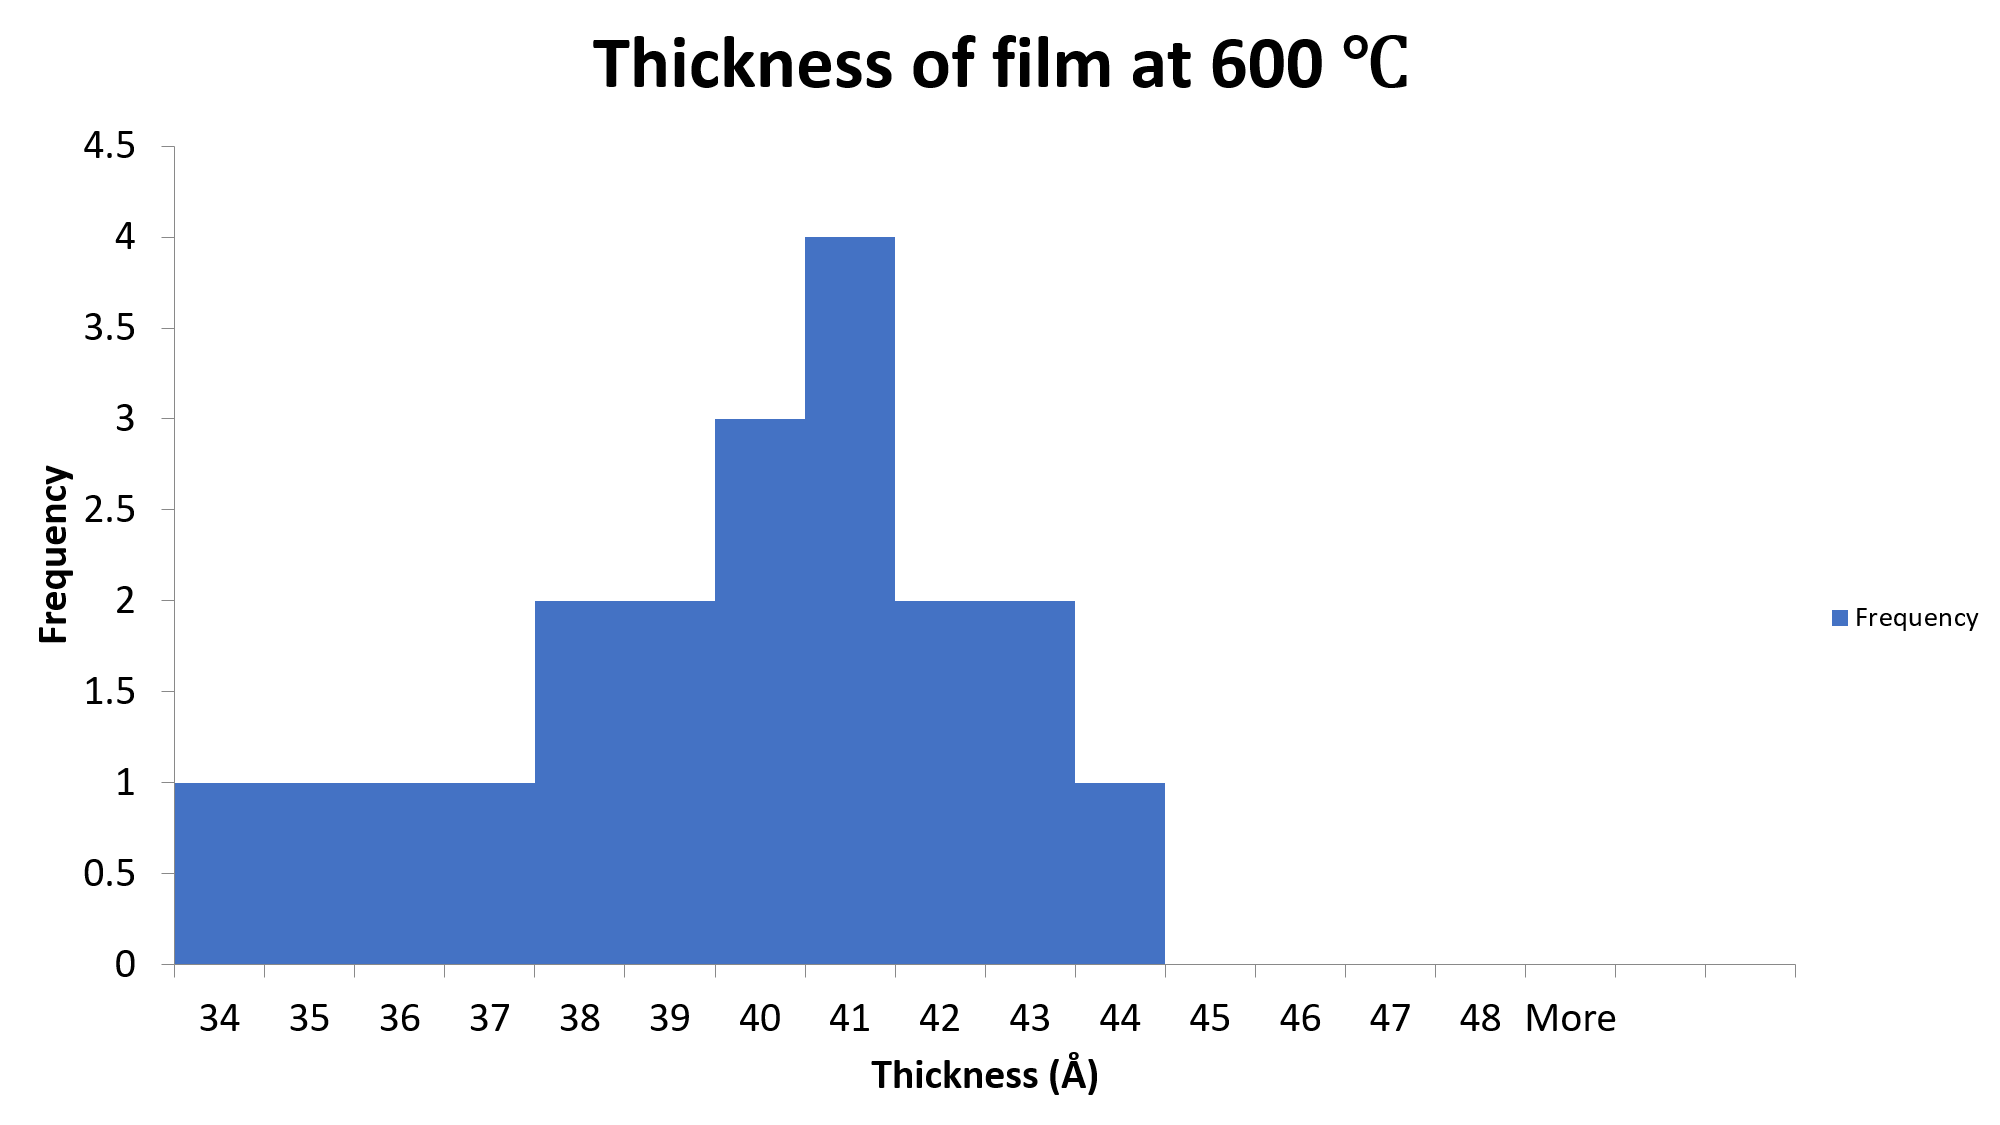
\includegraphics[width=\textwidth]{thicc600.png}
 \caption{INSERT CAPTION HERE}
 \label{thicc600}
\end{figure}

\begin{figure}[H]
 \centering
 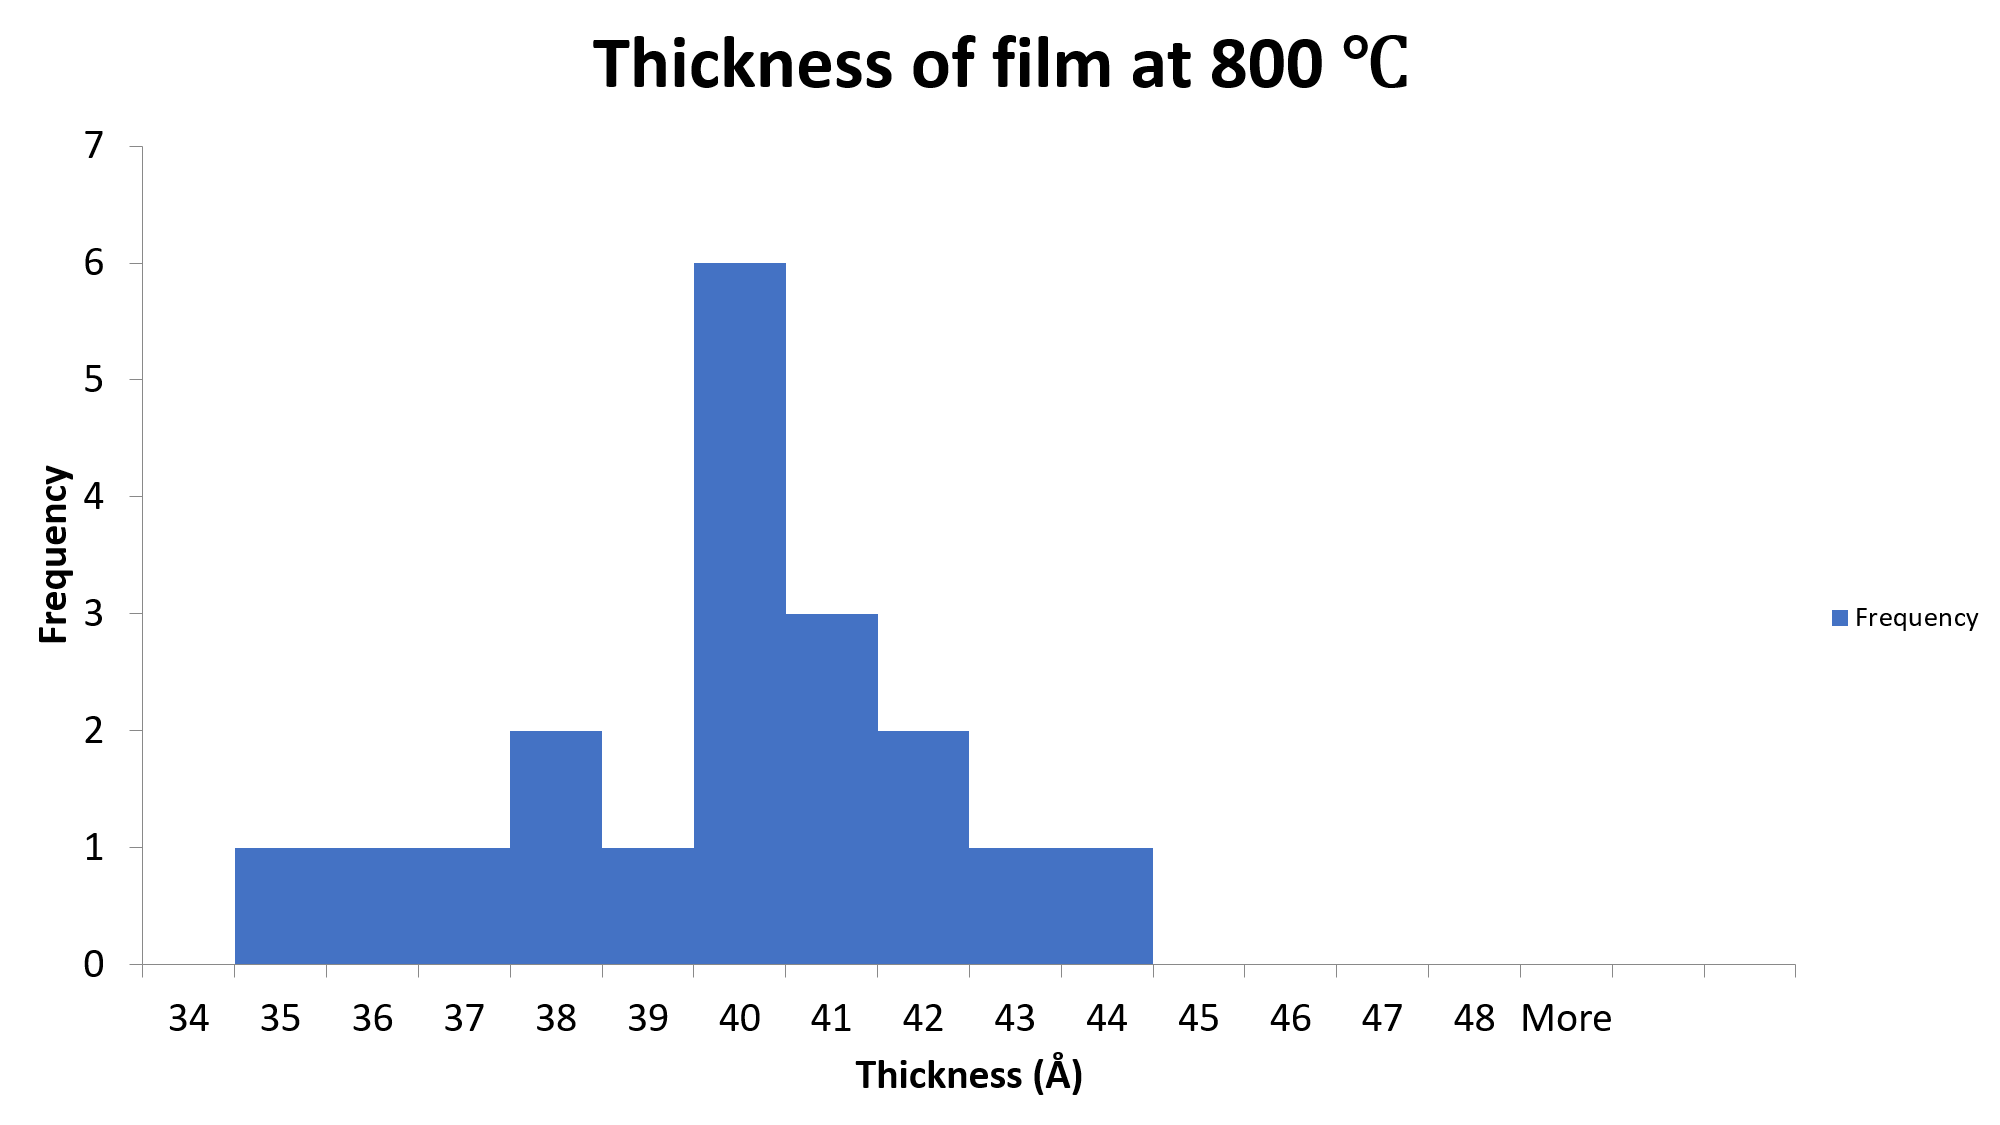
\includegraphics[width=\textwidth]{thicc800.png}
 \caption{INSERT CAPTION HERE}
 \label{thicc800}
\end{figure}

\subsection{Shapes}
All the histograms above appear to be slightly left-skewed. Figure
\ref{thicc400} appears to be very slightly left-skewed, while Figure
\ref{thicc600} appears to be a little more left-skewed. Figure \ref{thicc800}
also visually looks left-skewed as well. All histograms have one obvious peak,
but at first glance, Figure \ref{thicc800} might seem to have a second smaller
peak in bin 38, but upon further inspection, the frequency count only has a
difference of 1 compared to its surroundings, which does not seem significant
enough to count as a second peak. So, each histogram above is single-peaked.
There don’t seem to be any obvious outliers judging from the 3 histograms above.
When taking a step back and squinting, nothing seems to be visually away from
the bulk of the data.

\subsection{Centers and Spreads}
The first histogram (Figure \ref{thicc400}) has a center at bin 44, and a spread
(range) of 10. The second histogram (Figure \ref{thicc600}) has a center at bin
41 and a spread of 10 as well. The third histogram (Figure \ref{thicc800}) has a
center around 40, and has a spread of 9. For all 3 histograms, the means are
slightly less than their respective medians, or visually, the means are slightly
to the left of the medians, which seems to partially confirm the left skewness
of the histograms. (Although the difference betweem the medians and their
respective means is not huge.) The mean and median for each distribution can be
found in Tables \ref{tempmean} and \ref{tempquart} on page \pageref{tempmean}.


\subsection{Effect of Temperature on Thickness}
It would appear that increased temperature tends to result in overall lower
thickness of the films deposited. It can be noted that increasing the
temperature from \SI{400}{\celsius} to \SI{600}{\celsius} seems to result in a
more significant decrease in thickness overall, compared to the difference
between the process happening at \SI{600}{\celsius} and \SI{800}{\celsius}.

\section{Summary Statistics}

\subsection{Mean, Std. Deviation, Variance for each Temperature Level}

\begin{table}[H]
 \centering
 \begin{tabular}{c|c|c|c|}
  \multirow{2}{*}{Statistics} & \multicolumn{3}{c|}{Temperature Levels (\SI{}{\celsius})}             \\ \cline{2-4}
                              & 400                                                       & 600 & 800 \\ \hline
  Mean                        & 0                                                         & 0   & 0   \\ \hline
  Std. Deviation              & 0                                                         & 0   & 0   \\ \hline
  Variance                    & 0                                                         & 0   & 0   \\ \hline
 \end{tabular}
 \caption{My caption}
 \label{tempmean}
\end{table}


\subsection{Quartiles}

\begin{table}[H]
 \centering
 \begin{tabular}{c|c|c|c|}
  \multirow{2}{*}{Statistics} & \multicolumn{3}{c|}{Temperature Levels (\SI{}{\celsius})}             \\ \cline{2-4}
                              & 400                                                       & 600 & 800 \\ \hline
  Lower Quartile              & 0                                                         & 0   & 0   \\ \hline
  Median                      & 0                                                         & 0   & 0   \\ \hline
  Upper Quartile              & 0                                                         & 0   & 0   \\ \hline
  IQR                         & 0                                                         & 0   & 0   \\ \hline
 \end{tabular}
 \caption{My caption}
 \label{tempquart}
\end{table}

Wait check this
The 400  one doesn’t seem to match, but for 600  and 800 , the positions of the quartiles seem to support the conclusion that these histograms are left-skewed, since Q1 is further from the median than Q3 is.
\subsection{Mean \& Std. Deviation of Thickness at Each Pressure Value}

\begin{table}[H]
 \centering
 \begin{tabular}{c|c|c|c|}
  Pressure & Mean & Std. Deviation & Mean Change \\ \hline
  0        & 0    & 0              & 0           \\ \hline
  Average  &      &                & 0           \\ \hline
 \end{tabular}
 \caption{My caption}
 \label{pressurestat}
\end{table}

\section{Relationships}

\subsection{Thickness vs. Temperature}

\begin{figure}[H]
 \centering
 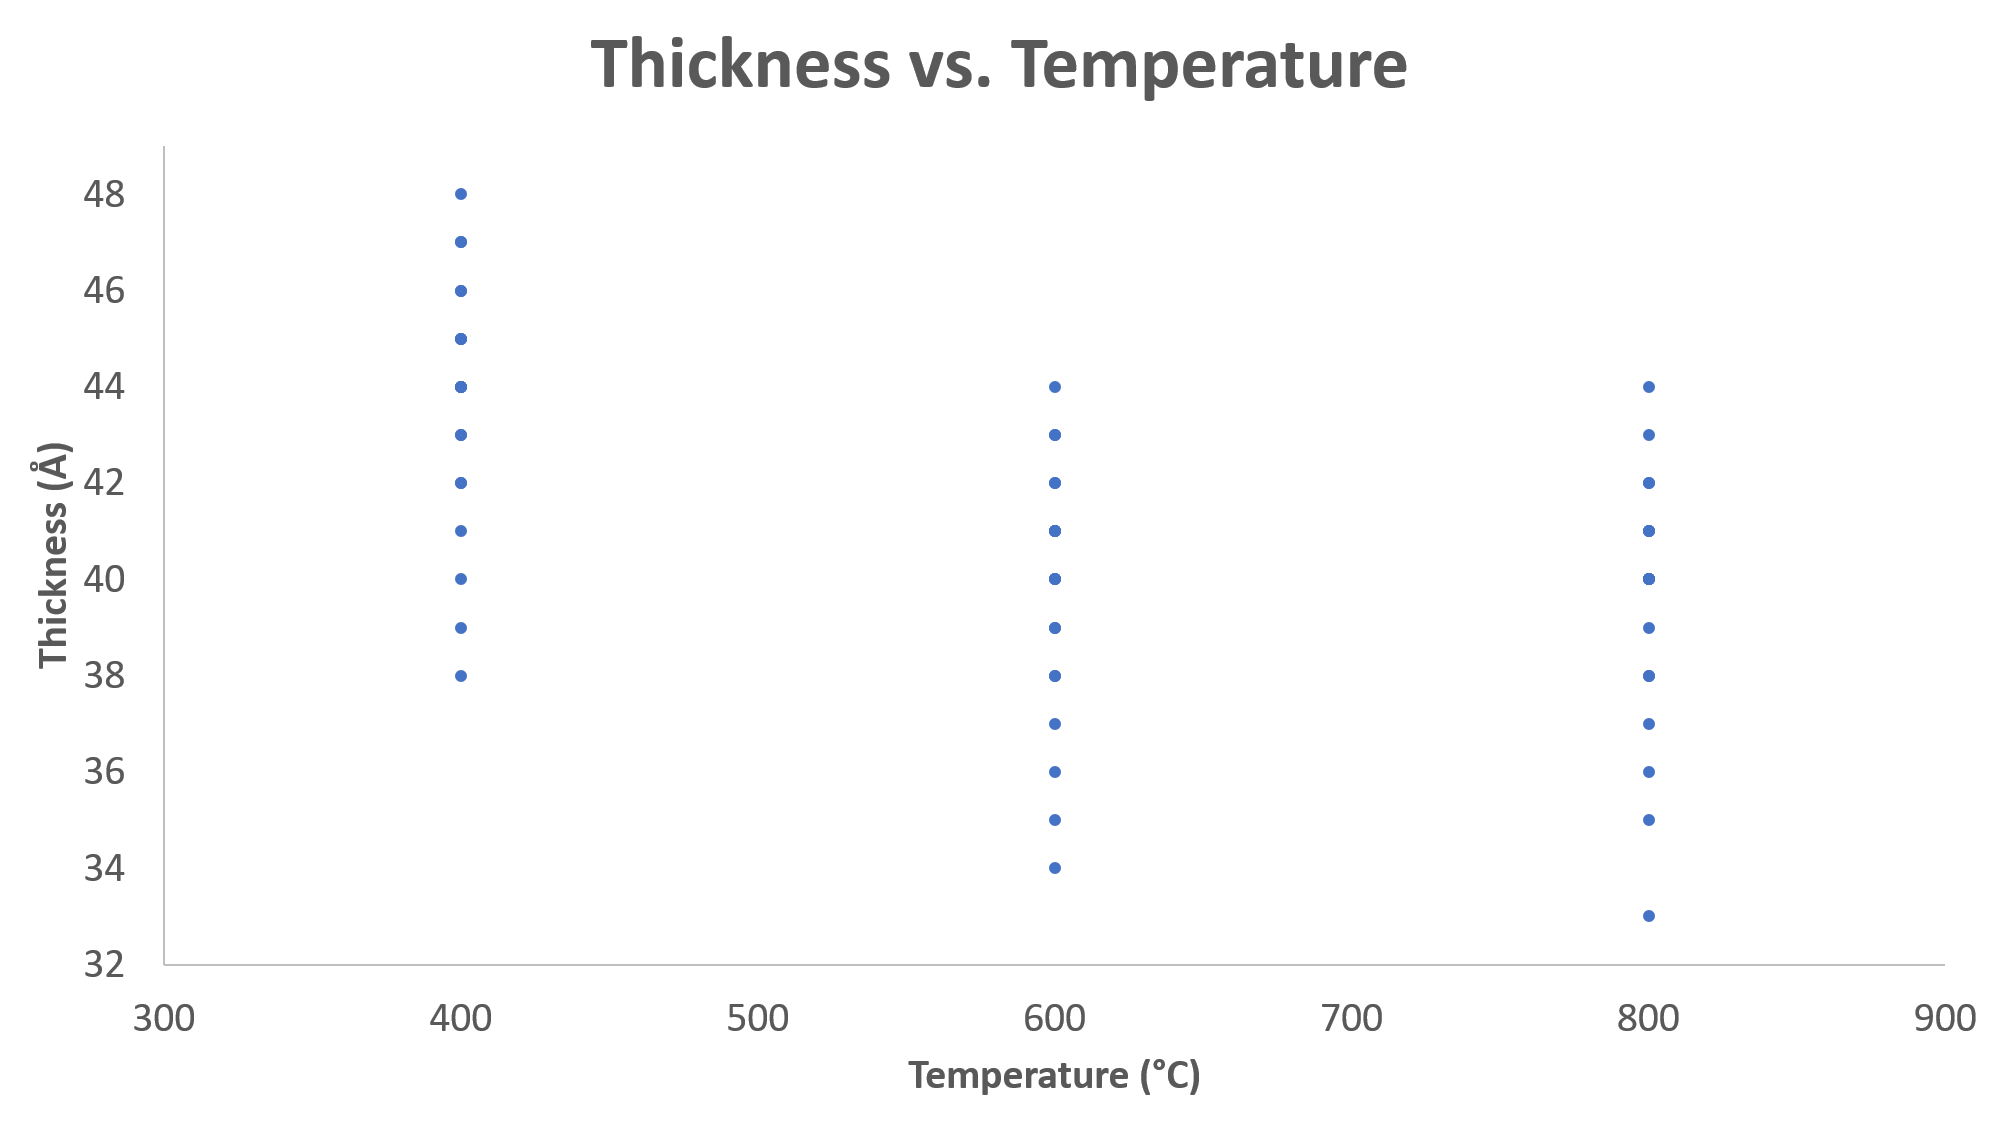
\includegraphics[width=\textwidth]{thiccvstemp.png}
 \caption{INSERT CAPTION HERE}
 \label{thiccvstemp}
\end{figure}

\subsection{Thickness vs. Pressure by Temperature}

\begin{figure}[H]
 \centering
 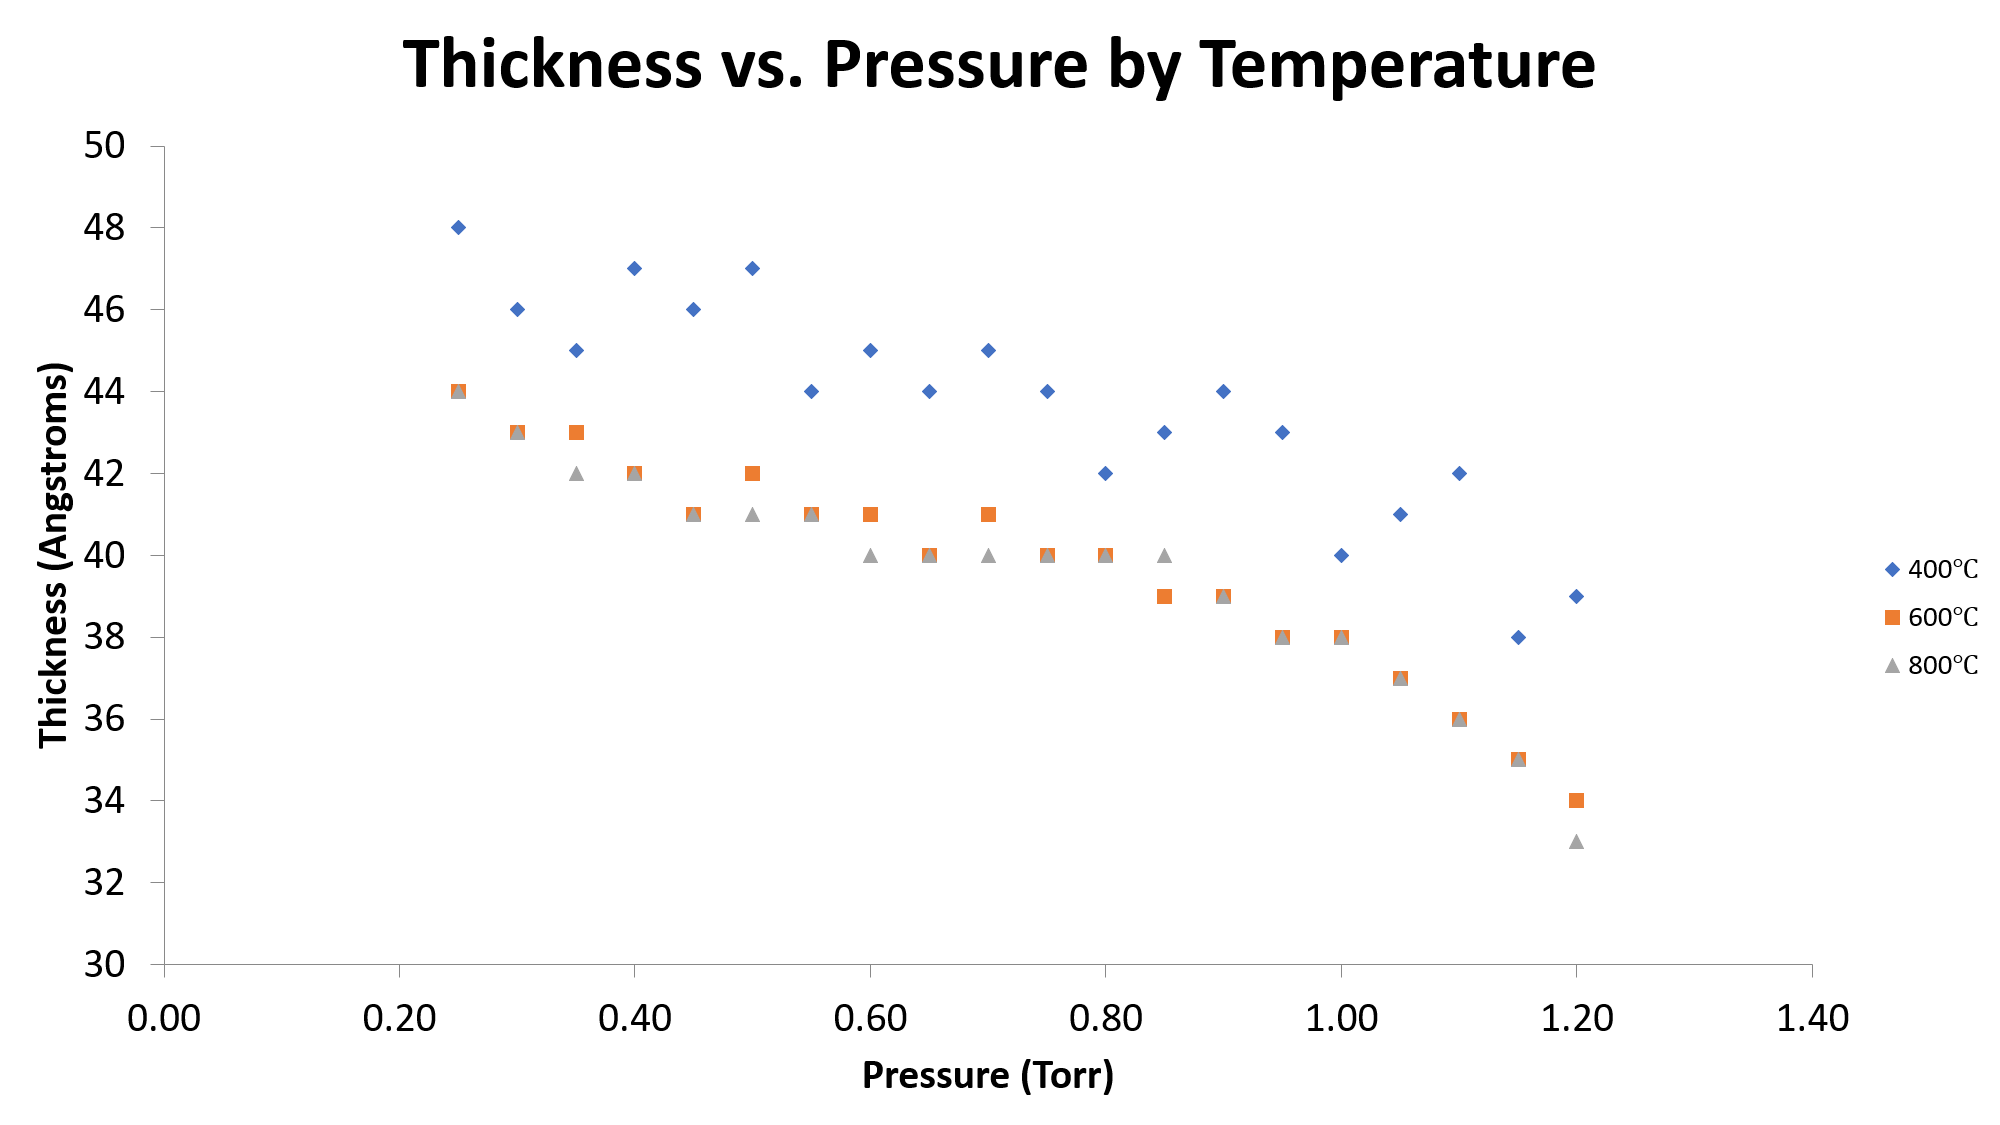
\includegraphics[width=\textwidth]{thiccvspressurebytemp.png}
 \caption{INSERT CAPTION HERE}
 \label{thiccvspressurebytemp}
\end{figure}


\subsection{Relationship Between Thickness and Pressure for each Temperature Level}

From Figure \ref{thiccvspressurebytemp}, we can see very clearly that as pressure
is increased, the thickness of the film decreases

\section{How should the temperature and pressure be selected to produce the thinnest possible film for the LPCVD process?}

From Figures \ref{thicc400}, \ref{thicc600}, and \ref{thicc800} we can see that
as the temperature is increased, the thickness of the film decreases, evidenced
by the bulk of the data shifting left in the histograms as the temperature
increases. By observing Tables \ref{tempmean} and \ref{tempquart}, we can see
that the mean and median averages for thickness also decrease as the temperature
is increased. We can also see this effect in Figure \ref{thiccvspressurebytemp},
where the effect is evidenced by the higher temperature lines
(\SI{600}{\celsius} \& \SI{800}{\celsius}) being lower than the
\SI{400}{\celsius} line. Next, when looking at the effect of pressure on the
thickness of the film deposited, we can see that in Table \ref{pressurestat},
the mean thickness decreases when the pressure is increased. This effect is also
seen in Figure \ref{thiccvspressurebytemp}, indicated by the negative slope of
each line. Therefore, in order to produce the thinnest possible film for the
LPCVD process, high pressure and temperature is desireable. It can be noted
however, that there may be diminishing returns as higher temperature and
pressure is used. For example, In Figures \ref{thicc400}, \ref{thicc600}, and
\ref{thicc800}, there is a more significant decrease in thickness by increasing
the temperature from \SI{400}{\celsius} to \SI{600}{\celsius} compared to the
decrease in thickness by increasing the temperature from \SI{600}{\celsius}
and \SI{800}{\celsius}.

\end{document}
